\documentclass[11pt]{article}
\usepackage[T1]{fontenc}
\usepackage[utf8]{inputenc}
\usepackage{graphicx}
\usepackage{minitoc}
\usepackage[french]{babel}
\usepackage[right=2.5cm, bottom=2.5cm,top=2.5cm, left=2.5cm]{geometry}
\title{\vspace{\fill} Interface et Multimédia \\ ~\textbf{IFT-215} \\~\\ Travail Pratique 3}
\author{Amandine Fouillet - 14 130 638 ~\\ Frank Chassing - 14 153 710 ~\\ Laurent Sénécal-Léonard - 14 143 484}
\date{\today \vspace{\fill}}
\begin{document}
\maketitle
\newpage

\tableofcontents
\listoffigures
\newpage
\section*{Introduction}


\section{Représentation globale de l'interface}
Dans cette premier partie, nous allons décrire les grandes lignes de l'interface ainsi que les liens entre les différentes fenêtres de l'application. Tous les éléments graphiques de l'interface décrit dans ce rapport seront représentés visuellement dans l'annexe de ce rapport. Les dessins de l'interface ont été réalisés avec un logiciel et représente notre application dans sa version OSX. Cependant, l'application pourra également être réalisée sur Windows et les supports mobiles comme iOS et Android. 
\subsection{Identité graphique}
Nous avons choisi de donner le nom "Awaï" à notre application. Ce nom rappelle le mot anglais "Away" qui signifie "Loin" et qui se rapporte à l'idée d'éloignement des familles qui utiliseront l'application. Nous avons changé le "y" par un "ï" pour ne pas utiliser le mot original et laisser un peu de mystère quand à la signification du nom. 

Pour le logo, nous avons choisi une icône d'avion. Simple à représenter, et pas trop encombrant, ce logo rappelle également la notion d'éloignement et de distance entre les utilisateurs.

Pour donner une cohérence entre toutes les fenêtres de l'application nous avons choisit de créer une petite identité graphique. Pour ce faire, nous avons décidé de reprendre des formes elliptique sur les différentes pages et d'appliquer un code couleur pastel (voir \textsc{Figure \ref{fig:codecouleur}}).
\subsection{La fenêtre de connexion}
Lors de la première utilisation, juste après son installation, l'application se lancera sur une fenêtre de connexion pour mettre à l'utilisateur de s'identifier et ainsi d'avoir accès à son espace personnel. Cette fenêtre comporte peu d'éléments mise à part le nom de l'application et son logo en haut au centre, trois boutons situés au milieu de la page : Connexion, Inscription et À Propos et enfin deux boutons iconiques en bas à gauche représentant les paramètres et l'aide. 

L'utilisateur pourra choisir de cliquer sur le bouton "Connexion" s'il est déjà inscrit à l'application, il rentrera alors ses identifiants et accédera à son espace. Au contraire, si c'est la première fois qu'il utilise l'application il sélectionnera "Inscription" et rentrera ses coordonnées pour se créer un compte. Enfin, il peut souhaiter en savoir plus sur l'application et aller explorer ce qui se trouve derrière le bouton "À Propos".  Les rôles des liens vers les paramètres et l'aide seront expliqués plus en détails dans la section \ref{par:aide}.

\subsection{Architecture de la fenêtre principale}
Sur la fenêtre principale, comme sur la fenêtre de 
\subsection{Lien entre les fenêtres}

\newpage
\section{Description des fonctionnalités}
\subsection{La communication}
\subsection{Le partage de photos}
\subsection{L'emploi du temps}
\subsection{Le suivi des dépenses}
\subsection{La carte du monde}
\subsection{Les paramètres et l'aide en ligne}\label{par:aide}

\newpage
\section*{Conclusion}

\newpage
\section*{Annexes}
\begin{figure}[hbtp]
        \centering 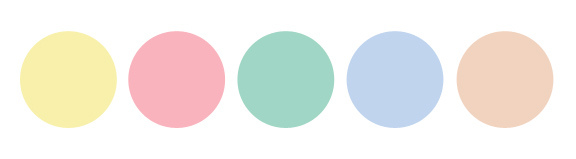
\includegraphics[scale=0.6]{Modelisation/Couleurs/pastels.jpg}
        \caption{Code couleur}
	\label{fig:codecouleur}
\end{figure}
\begin{figure}[hbtp]
    \begin{minipage}[b]{0.4\linewidth}
        \centering 
\includegraphics[scale=0.43]{Modelisation/connexion.png}
        \caption{Fenêtre de connexion}
	\label{fig:connexion}
    \end{minipage}\hfill
    \begin{minipage}[b]{0.48\linewidth}
        \centering 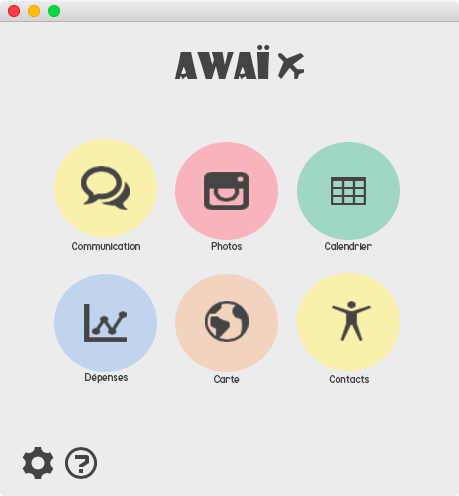
\includegraphics[scale=0.43]{Modelisation/awai.png}
       \caption{Fenêtre principale}
\label{fig:principale}
    \end{minipage}
\end{figure}
\begin{figure}[hbtp]
    \begin{minipage}[b]{0.4\linewidth}
        \centering 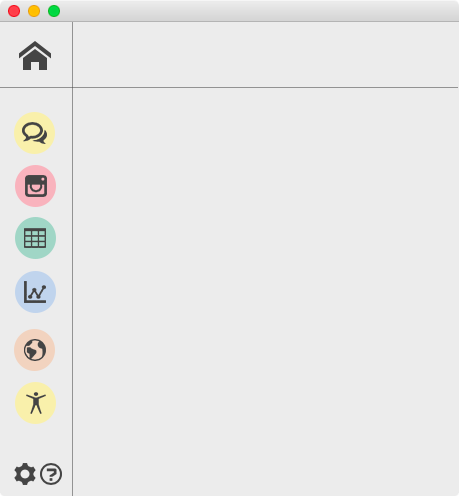
\includegraphics[scale=0.43]{Modelisation/base.png}
        \caption{Base de l'interface}
\label{fig:base}
    \end{minipage}\hfill
    \begin{minipage}[b]{0.48\linewidth}
        \centering 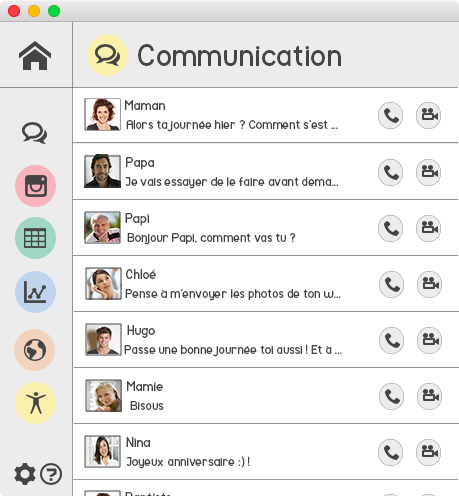
\includegraphics[scale=0.43]{Modelisation/communication.png}
        \caption{Gestion des communications}
        \label{fig:communication}
    \end{minipage}
\end{figure}
\begin{figure}[hbtp]
    \begin{minipage}[b]{0.4\linewidth}
        \centering 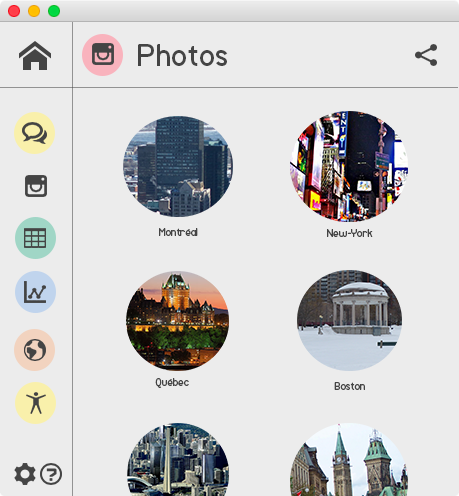
\includegraphics[scale=0.43]{Modelisation/photos.png}
        \caption{Gestion des photos}
                \label{fig:photos}
\label{fig:base}
    \end{minipage}\hfill
    \begin{minipage}[b]{0.48\linewidth}
        \centering 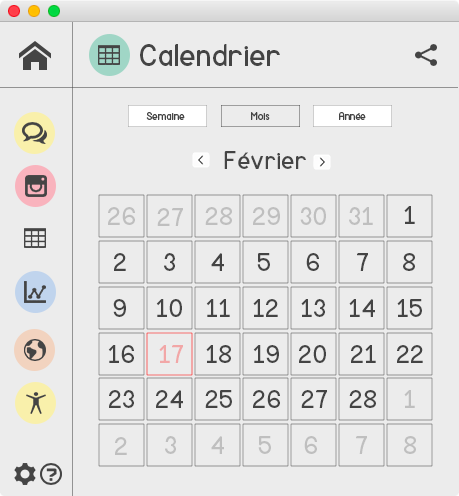
\includegraphics[scale=0.43]{Modelisation/calendrier.png}
        \caption{Gestion du calendrier}
        \label{fig:calendrier1}
    \end{minipage}
\end{figure}
\begin{figure}[hbtp]
    \begin{minipage}[b]{0.4\linewidth}
        \centering 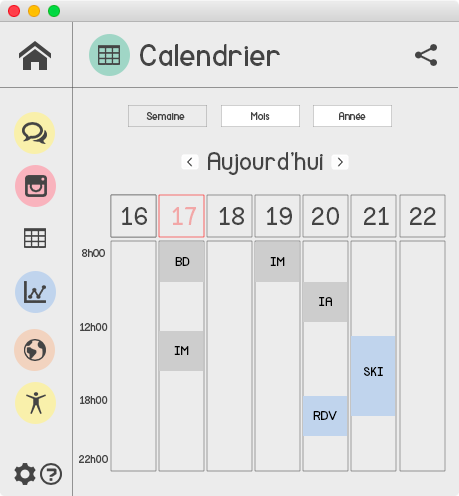
\includegraphics[scale=0.43]{Modelisation/calendrier2.png}
        \caption{Gestion du calendrier}
                \label{fig:calendrier2}
\label{fig:base}
    \end{minipage}\hfill
    \begin{minipage}[b]{0.48\linewidth}
        \centering 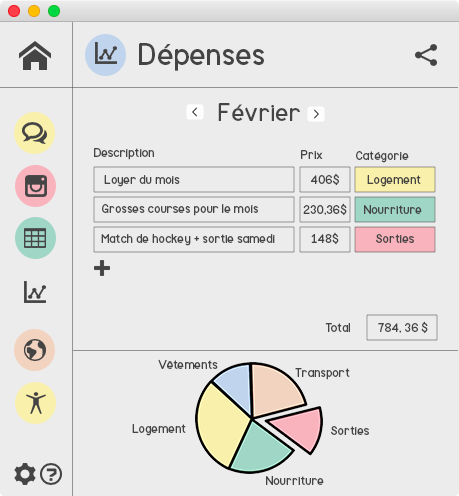
\includegraphics[scale=0.43]{Modelisation/depenses.png}
        \caption{Gestion des dépenses}
         \label{fig:depenses}
    \end{minipage}
\end{figure}
\begin{figure}[hbtp]
    \begin{minipage}[b]{0.4\linewidth}
        \centering 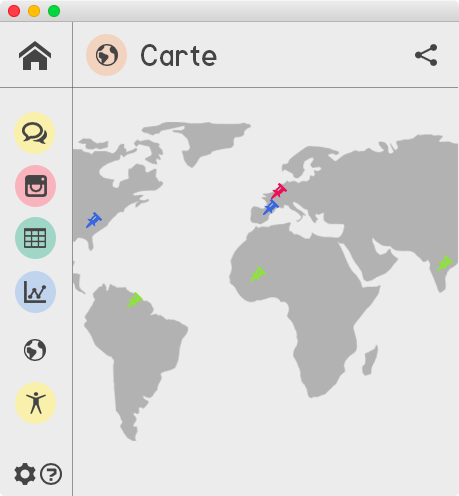
\includegraphics[scale=0.43]{Modelisation/carte.png}
        \caption{Gestion de la carte}
                \label{fig:carte}
\label{fig:base}
    \end{minipage}\hfill
    \begin{minipage}[b]{0.48\linewidth}
        \centering 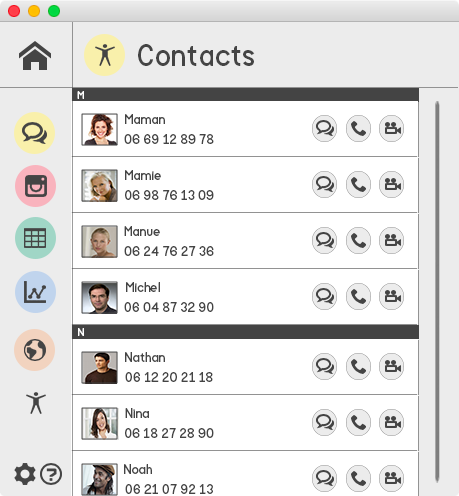
\includegraphics[scale=0.43]{Modelisation/contact.png}
        \caption{Gestion des contacts}
         \label{fig:contact}
    \end{minipage}
\end{figure}


\end{document}